\chapter{Antecedentes}

A principios del milenio, el grupo GITEM realizó un estudio para abordar problemas puntuales en la implementación de servicios médicos prestados a través de medios teleinformáticos en el Distrito Capital\cite{aparicio2000}:

\begin{quote}
“En el momento no existe un diagnóstico real sobre los servicios requeridos en el área de telemedicina, razón suficiente para iniciar un trabajo de campo que establezca la situación actual de servicios médicos y la demanda real, así como la posibilidad de conocer a corto, mediano y largo plazo cuáles serían los costos de inversión que permitirían dar soluciones al problema  de cobertura.

La socialización del conocimiento alrededor de las tecnologías aplicadas al desarrollo de la medicina, es uno de los valores que lleva al éxito de soluciones efectivas en el sector salud, por tal motivo es necesario desarrollar un plan de alfabetización en el sector salud y en el sector gubernamental y académico.

En el país no existen estrategias de investigación en esta área del conocimiento para llevar a cabo un estudio real que permita dar el paso a soluciones verdaderas sobre desarrollo tecnológico o experimental para poder implementar centros de investigación en Telemedicina.

La Universidad Distrital tiene el recurso humano, el conocimiento y la experiencia científica y tecnológica, capaz de dar soluciones tangibles a estas necesidades; unida al conocimiento y experiencia de entidades como clínicas y hospitales  y con la participación de operadores de comunicaciones, puede desarrollar soluciones efectivas a los problemas de salud que afronta la sociedad colombiana.”
\end{quote}

Los resultados obtenidos fueron recopilados en extensos tomos en formato físico y digital. Luego de los primeros análisis, se observó que los reportes no tenían una estructura documental coherente ni un modelo de información que los caracterizara. Este hecho, a la par con el ingreso de entidades al estudio, aumentó la complejidad a la hora de generar estudios comparativos o de apoyo a la toma de decisiones. Se evidenciaron casos de información faltante o innecesaria para el proyecto. Como consecuencia, al ser el objeto de estudio intrínsecamente dinámico, cualquier cambio de la condiciones iniciales no se ve reflejado y la información queda desactualizada rápidamente. En ese escenario, la labor de articular información de las organizaciones suponía un proceso lento por lo cual la estrategia de gestión de información empleada en el estudio comenzó a mostrar debilidades.

Respondiendo a este contexto problémico se creó al interior del grupo un proyecto denominado \textbf{Sistema para la Caracterización de Nodos Potenciales de Redes de e-salud}, que en sus primeras fases de desarrollo ha dado solución parcial al marcar las pautas hacia la integración de información para el \textbf{GITEM}. En paralelo el grupo de investigación implementó, en convenio con \textit{Colciencias}, el Sistema de Referencia y Contrarreferencia para el Distrito Capital, utilizando herramientas de desarrollo propietarias específicamente el middleware .NET de Microsoft con lo que el grupo adquirió experiencia en la desarrollo de aplicaciones siguiendo metodologías efectivas para la construcción de software. Así las cosas, el estudio base generó una \textit{instantánea} de la capacidad de la red de salud del distrito para el emprendimiento de proyectos de eSalud pero no se logró un sistema que permitiera \textit{observar} la evolución de dicha capacidad - o tomar otras instantáneas a través del tiempo.

\section{Sistema para la Caracterización de Nodos Potenciales de Redes de e-salud}

El proyecto que se describe en este documento surge de la necesidad de contar con un espacio común de información que permita valorar la capacidad de las instituciones que pertenecen a una red de salud y ofrecer un mecanismo de observación, intercambio, análisis y colaboración entre equipos de consultoría y diseño de redes de eSalud. El proyecto - cuyo nombre de desarrollo es OpenSITEM, pretende brindar una plataforma tecnológica para que grupos de trabajo especializados puedan integrar (cargar, almacenar, analizar, categorizar, comparar) los datos que les permitan responder inquietudes tales como:

\begin{itemize}
 \item ¿cuáles son las necesidades de servicios de la población que atiende la institución?
 \item ¿cuáles son las características de la redes eléctricas, de telecomunicaciones, de servicios médicos, de profesionales y de equipos médicos de la institución?
 \item De un grupo seleccionado de instituciones, ¿cuál es la de mayor potencial para la prestación de un servicio de eSalud?
 \item ¿cuál es la capacidad de un proveedor de telecomunicaciones para atender la demanda de un determinado servicio en una zona específica?
\end{itemize}

OpenSITEM se presenta como un sistema federado de aplicaciones de código abierto que, en conjunto, ofrecen herramientas para contestar estas u otras preguntas relacionadas. Si bien el desarrollo de cada componente no se ha abordado por el grupo, la contribución innovadora radica tanto en la arquitectura como en el motor de integración que conducen a un modelo de utilidad que permite la interoperabilidad novedosa de aplicaciones preexistentes en un nuevo dominio de negocio, con potencial de ser utilizado en procesos de diseño y planeación de sistemas de eSalud.

El proyecto ha pasado por varias fases que han correspondido a etapas dentro de un proceso de investigación emergente. El producto ha evolucionado de un simple sitio web construido 100\% \textit{in - house}, a una solución federada - centrada en una arquitectura y guiada por casos de uso - que recoge los aspectos de calidad definidos por cada uno de sus componentes y del motor de integración. A continuación se describen brevemente cada una de las fases:

\subsection{SITEM – Fase I}

El objetivo de esta fase fue la definición de un modelo de información que permitiera la gestión de resultados del estudio de campo. A partir de dicho modelo se presentó la recomendación de definir un sistema informático que permitiera gestionarlo. Con los resultados de esta fase se encontró \textit{un costo de oportunidad adecuado debido a que en la actualidad ningún portal se especializa en el proceso de diagnóstico de capacidad para la implementación de proyectos de eSalud.}

Los alcances y logros efectivos de esta fase fueron:

\begin{itemize}
\item Descripción base del Modelo de Información.
\item Propuesta de Desarrollo de portal especializado.
\item Bosquejo de la Arquitectura general del Sistema.
\item Integración del SITEM dentro de los proyectos del grupo, entendiéndolo como una plataforma tecnológica para soportar grupos de trabajo que constituyan un \textit{observatorio} multitemporal de los nodos que constituyen las redes de salud, con iras a servir de referente para la medición de capacidad para el despliegue - o seguimiento, a proyectos de eSalud.
\item Estudios sobre filosofía de Software Libre y el movimiento del código abierto.
\item Construcción de un Prototipo de baja funcionalidad conocido como SITEM versión 0.1, bautizada internamente como \textbf{Kauil}. Este prototipo se construyó totalmente por los integrantes del grupo y aunque estuvo al aire durante dos años nunca alcanzó una versión estable ni sus características de calidad fueron evaluadas,
\end{itemize}

Para la construcción del prototipo se experimentó un proceso de desarrollo ágil considerando los principios de Kanban \cite{anderson2016}. Con algo de esfuerzo se apropiaron los valores y algunas técnicas de trabajo propuestas por el método. Sin embargo, ciertas especificidades del proyecto condujeron a un entorno de riesgo que no fue posible gestionar. Principalmente se priorizaron como principales causas:

\begin{itemize}
  \item Escasos recursos de personal, financieros y técnicos. Durante esta fase el grupo de investigación priorizó el estudio de campo por lo cual SITEM tenía asignado solo dos integrantes.
  \item Competencias y habilidades no homogéneas entre participantes. Esto condujo a inversión de tiempo en capacitación, aún cuando un supuesto era que al tener estudiantes de últimos semestres estos tendrían formación en ingeniería de software y desarrollo de sistemas.  
  \item Bajo tiempo de permanencia de los integrantes. Con un promedio de retención inferior a 0.5 años y un nivel de inmersión promedio de 2 horas/día.
  \item Inexistencia de mecanismos de transferencia de conocimiento. Teniéndose como técnica única la capacitación basada en clase magistral por parte de integrantes experimentados.
  \item Incorrecta disciplina de requisitos y arquitectura.
  \item Enfoque en donde el código fuente se consideraba el único producto. Esta visión impidió que el grupo de trabajo tuviese un conjunto de artefactos que evolucionara de manera consistente. 
\end{itemize}

\begin{figure}
 \centering
 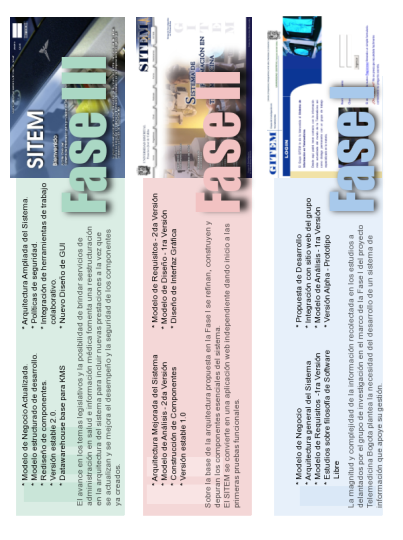
\includegraphics[width=142mm, height=190mm]{fase_sitem.png}
 \caption{Fases transcurridas en el desarrollo del SITEM}
 \label{fase_sitem}
\end{figure}

\subsection{SITEM – Fase II}

Conscientes de la oportunidad de negocio se evaluaron los resultados y experiencias de la primera fase. Un análisis de riesgo permitió definir estrategias de tratamiento que incluyeron los siguientes aspectos:

\begin{itemize}
 \item Adopción de un método de desarrollo guiado por casos de uso, centrado en la arquitectura, iterativo e incremental.
 \item Fortalecimiento del modelo de transferencia de conocimiento a partir de la creación de objetos de aprendizaje.
 \item Uso de marco de trabajo (frameworks).
 \item Definición de lineamientos de trabajo.
 \item Enfoque en la interoperabilidad.
 \item Limitación del dominio de negocio a los nodos de entidades de salud en sus redes eléctricas y de telecomunicaciones.
 \item Liberación del código para facilitar el desarrollo colaborativo.
\end{itemize}

Con la experiencia se comprobó la máxima de Larman \cite{larman2003} : “Rápido, barato, bueno: elija dos cualquiera”. Dejando a un lado las esperanzas utópicas, sacrificamos la rapidez en que versiones estables del proyecto habrían de ver la luz.

La metodología permitió elegir a OpenUP como el método de trabajo y se declaró la fase II como etapa para desarrollar una visión base, planificar el proyecto, preparar el ambiente de trabajo, definir el modelo base de requisitos y lograr acuerdos acerca del enfoque técnico que debe regular el desarrollo.

Los alcances de esta fase fueron:
\begin{itemize}
\item Elaboración de la visión general del proyecto.
\item Aprobación del plan general del proyecto para las fases II (inicio), III (elaboración y construcción) y IV (transición).
\item Modelo base de Requisitos.
\item Bosquejo de la Arquitectura del Sistema.
\item Modelo de Información - Segunda Versión.
\item Definición de los requisitos mínimos del ambiente de trabajo.
\end{itemize}

\subsection{OpenSITEM – Fase III}

La fase III se corresponde a las fases de elaboración y construcción definidas en OpenUP \cite{balduino2010}. Para concretar la visión el grupo toma una decisión arquitectónica importante y concentra su esfuerzo en un motor de integración de aplicaciones, cuyo objetivo es la federación de sistemas existentes de software libre o código abierto (FLOSS). De esta manera se logra un mayor nivel funcional del que se había poder alcanzado de seguir con un desarrollo 100\% in-house. Con esto se busca el aseguramiento de la calidad en el desarrollo, la interoperabilidad, escalabilidad y el uso extensivo de soluciones consolidadas de software libre o de código abierto. 

Para recalcar la adopción de la filosofía del código abierto todo el código generado se gestiona en un repositorio público en la plataforma GitHub. De manera complementaria y considerando el producto de manera integral, se elaboran diferentes artefactos y se formaliza las áreas de capacitación a partir de ciclos genéricos de transferencia de conocimiento apoyados en tecnologías de la información.

Es precisamente esta fase la que da vida a este documento, a una arquitectura emergente y una versión 1.0 del sistema denominada \textit{OpenSITEM}, con la que el grupo entrega un sistema complejo constituido por un motor de federación (basado en OpenSARA, un framework de desarrollo para aplicaciones web desarrollado por el grupo) que articula las herramientas externas Knowage, ERPNext, Alfresco Community, CAMUNDA y OpenProject, así como varias herramientas propias tales como:

\begin{itemize}
\item Sistema Integrado de Evaluación
\item Sistema de Gestión de Redes de Práctica y Colaboración
\item Sistema de agentes notificadores y de recomendación
\item Sistema de Información Geográfica 3D.
\end{itemize}

De esta forma OpenSITEM propone una solución que abarca diferentes dominios pero con capacidad de adaptación para el propósito específico de las necesidades del proyecto \textit{Sistema Federado de Aplicaciones para la Caracterización de Proyectos de e-salud}.


\begin{figure}
 \centering
 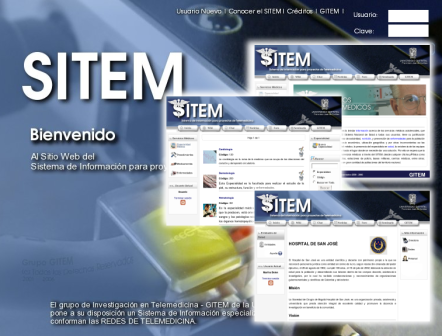
\includegraphics[width=156mm, height=118mm]{pagina_principal.png}
 \caption{Sistema de Información para la Caracterización de Proyectos de eSalud. Interfaz de Usuario en la Fase III}
 \label{sitem_faseIII}
\end{figure}